\subsection{Язык \logiql}
\label{sec:technology:logiql}

Для создания платформы, подходящей под описание в предыдущей главе, жизненно важно был необходим свой универсальный язык, с помощью которого можно писать подобные программы. Поскольку основной целью системы является унификация модели программирования для приложений принятия решений, был  разработан единый экспрессивный декларативный  язык \logiql. Его характерные черты:

\begin{itemize}
  \item Расширяет возможности \datalog, который использовался как язык запросов. Синтаксически очень похож на него, оперирует такими же терминами (предикаты). На нем можно писать запросы, хранимые процедуры, триггеры и тп. На основе \datalog уже разработаны такие индустриальные системы, как Yedalog (Google) \cite{yedalog}, Datomic \cite{datomic}
  \item Позволяет читать код бизнес-консультантам и понимать, что там происходит. Очень низкий порог вхождения для его понимания.
  \item Многие известные языки выполняются сверху-вниз и слева-направо. Редкое явление, но \logiql так не делает. Фактически, программист даже не задумывается о том, в каком порядке выполняется его код, самое главное, что \emph{он будет выполнен тогда, когда это действительно надо}. Такое свойство дает гибкость в \emph{автоматическом} параллелизме выполнения запросов, обновления состояния базы данных и тп.
\end{itemize}

\begin{figure}
	\centering
	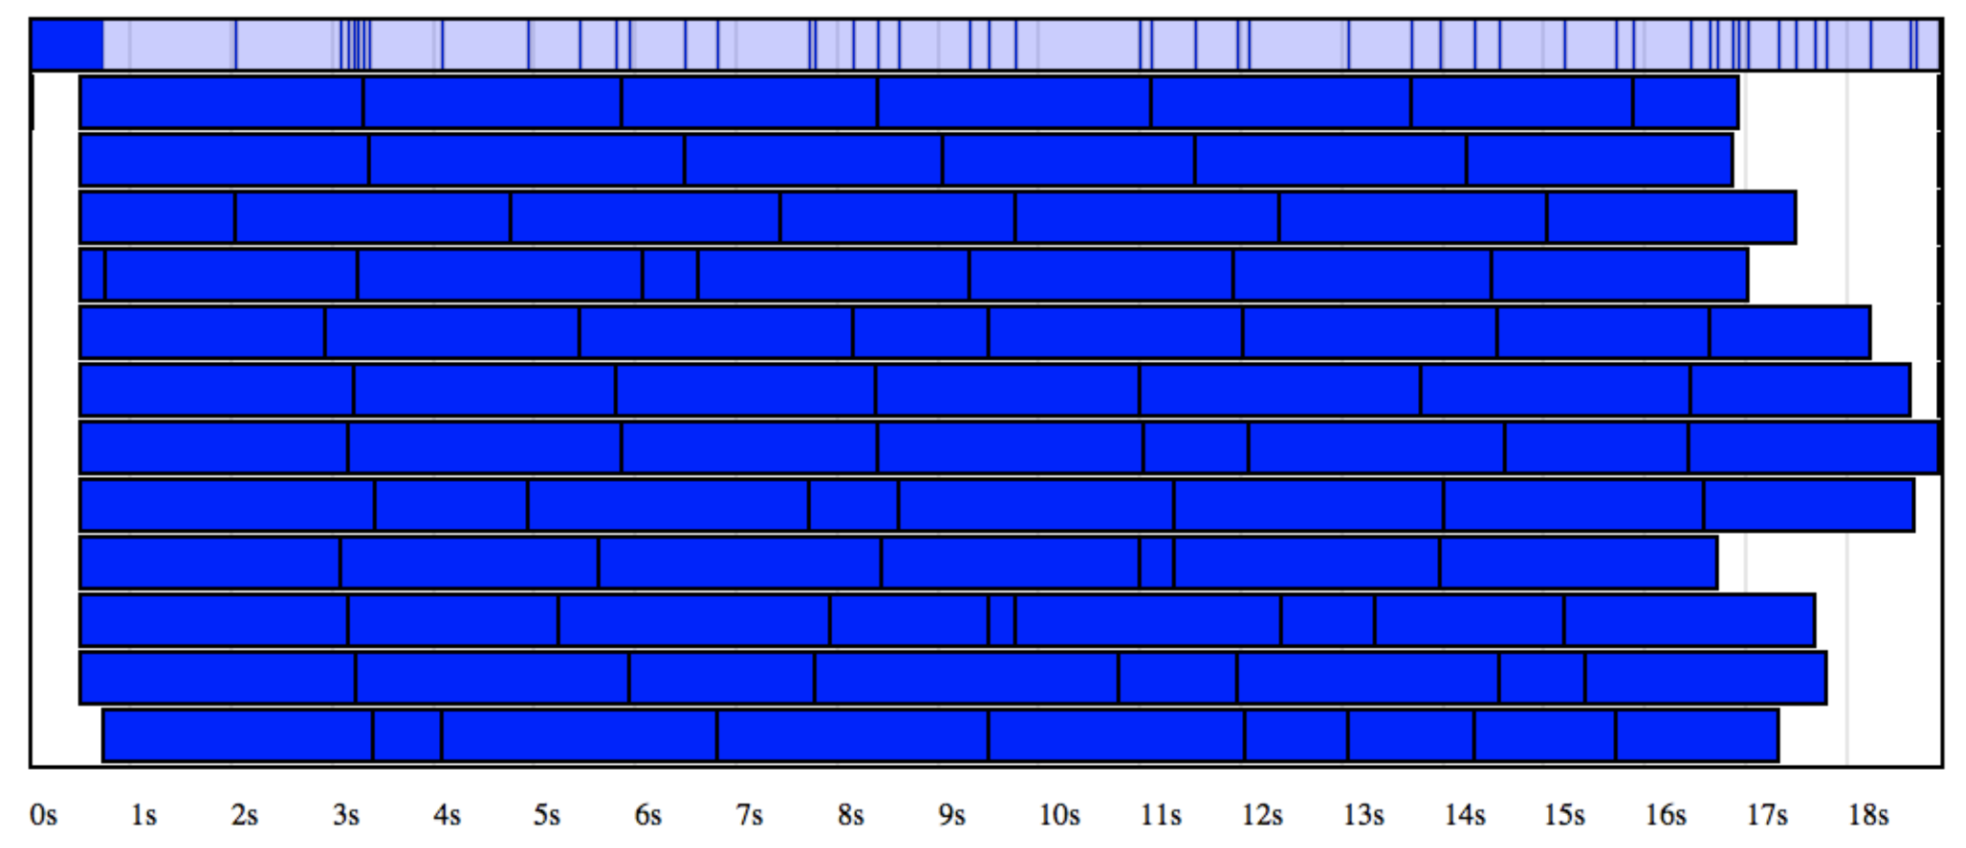
\includegraphics[scale=0.2]{query_parallel.png}
	\caption{Параллельное выполнение сложного запроса \cite{query_parallel_execution}}
	\label{fig:technology:logiql:query_parallel}
\end{figure}

Базой языка является бивалентность (или двухзначная логика, когда утверждение либо принимает либо truth значение, либо false), и множество. Все транзакции выполняются на самом высоком уровне изолированности, при котором параллельные транзакции не подвержены эффекту "фантомного чтения". Исторически при таком подходе простота и правильность шли бок о бок с проблемами расширяемости и производительности. Но разработчикам \logiql удалось этого избежать, наложив дополнительные ограничения и усовершенствовав некоторые возможности:

\begin{itemize}
  \item 6-я нормальная форма \cite{intro_into_db}. Поэтому нет \lstinline{null} - это следует из бивалентности, два значения проще обрабатывать, чем три. Кроме этого, это помогает избежать сложных ошибок. \cite{three_valued_logic}
  \item Простота в изменении схемы базы данных. Чем больше разработчику нужно вносить корректировки в схему, тем менее устойчива она становится. Добавление и удаление новых сущностей и отношений в \logiql приложение требует значительно меньше вмешательства и времени бездействия системы.
  \item Уменьшает количество просматриваемых атрибутов при выполнении запроса в сравнении с хранением большой таблицы благодаря меньше информационной энтропии.
\end{itemize}

У 6 нормальной формы есть один недостаток: запросы, хоть и затрагивают меньшее количество атрибутов, но просматривают большее количество связей. Поэтому операция выборки данных часто проходится по многим связям, выполняя одновременно много операций \join, суживая результаты по многим условиям. В связи с этим необходимы новые наработки в области алгоритмов для этой операции. В платформе используется \emph{Leapfrog trie-join} алгоритм \cite{leapfrog_tree_join_algo}. Подробнее можно прочитать в ссылке описания, общие сведение на архиве. Этот алгоритм хорош тем, что обгоняет алгоритмы AGM и NPRR асимптотически для большого круга операций, которых достаточно для использования в базе данных. Он также применим к таким БД структурам данных, как B-деревья. Для некоторого набора операций асимптотика составляет $O(n\log{n})$, в то время как указанные алгоритмы работают за $O(n^{1.3})$.

Чтобы интуитивно понять этот алгоритм и почему одновременный \join выгоднее, чем попарный, рассмотрим следующую ситуацию (рисунок \ref{fig:technology:logiql:leapfrog_trie_join_algo_intuition}). Пусть множества \lstinline{A(x)}, \lstinline{B(x)} и  \lstinline{C(x)} пересекаются в приведенном порядке. Пусть также каждая клетка содержит означает количество записей по соответствующей категории в одну тысячу (то есть множество  \lstinline{A(x)} содержит по тысяче записей в магазине 1 и магазине 2, \lstinline{C(x)} - по тысяче в магазине 1 и магазине 3). Любое попарное пересечение генерирует $500$ записей, в то время как одновременное пересечение не дает никаких результатов. Это упрощает процесс фильтрации, "охватывая" значительно меньшее количество записей.

\begin{figure}
	\centering
	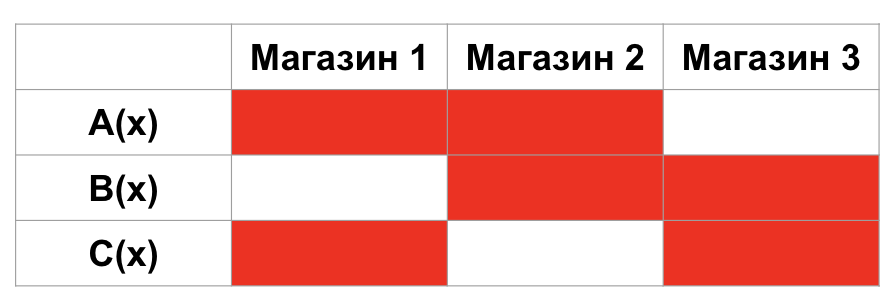
\includegraphics[scale=0.5]{leapfrog_trie_join_algo_intuition.png}
	\caption{Пример пересечения множеств \lstinline{A(x)}, \lstinline{B(x)}, \lstinline{C(x)}}
	\label{fig:technology:logiql:leapfrog_trie_join_algo_intuition}
\end{figure}


\subsubsection{Определение предикатов}
\label{sec:technology:logiql:predicates}

Для более наглядного представления об этом языке следует разобрать пример из предыдущей главы.

\begin{lstlisting}[language=Prolog]
sales_u(product, store, day, unit) ->
  string(product),
  string(store),
  datetime(day),
  int(units).
\end{lstlisting}

Или, аналог \sql:

\begin{lstlisting}[language=SQL]
CREATE TABLE sales_u
(
  product VARCHAR(15) NOT NULL,
  store VARCHAR(20) NOT NULL,
  day DATETIME NOT NULL,
  unit INT NOT NULL
);
\end{lstlisting}

Здесь \lstinline{sales_u} является предикатом - аналог термина «таблица» в
\sql. Из записи видно, что этот предикат состоит из 4 колонок, типы которых \lstinline{string}, \lstinline{string}, \lstinline{datetime}, \lstinline{int} соответственно. Если быть точнее, то определение должно быть дано немного другим образом: если в предикате \lstinline{sales_u} есть некоторая запись, то это означает, что тип значения в первой колонке должен быть \lstinline{string}, второй – \lstinline{string}, третьей – \lstinline{datetime}, и, наконец, четвертой – \lstinline{int}. Об этом свидетельствует знак импликации (\lstinline{->}). При этом стоит отметить, что здесь важен лишь порядок следования значений в предикате, \lstinline{product}, \lstinline{store}, \lstinline{day}, \lstinline{units} – это лишь псевдонимы значений на этих позициях в данном контексте. Это, как упоминалось ранее, определение схемы.

\subsubsection{Жизненный цикл транзакции}
\label{sec:technology:logiql:transaction}

Как и язык \sql, \logiql имеет свой жизненный цикл транзакций. Согласно Википедии \cite{transaction_definition} транзакция – группа последовательных операций с базой данных, которая представляет собой логическую единицу работы с данными. Транзакция может быть выполнена целиком и успешно, соблюдая целостность данных и независимо от параллельно идущих других транзакций (рисунок \ref{fig:technology:logiql:query_parallel}), либо не выполнена вообще, и тогда она не должна произвести никакого эффекта.
В \logiql также имеется понятие \emph{workspace} (рабочее пространство) – своеобразное пространство имен, хранилище для особых предикатов. В этом пространстве содержатся как данные, так и программный код, который был либо был написан разработчиком, либо сгенерирован системой. Рисунок \ref{fig:technology:logiql:transaction} показывает упрощенную версию жизненного цикла этого пространства \cite{query_language_for_smart_db}.
Изначально надо создать \emph{workspace}. Изначально он будет содержать только стандартный набор системных предикатов. Созданный \emph{workspace} можно изменять через транзакции.
Чтобы полнее разобраться в том, как выполняются транзакции, стоит дать определения понятиям блоков и стадий. Блок – это единица кода \logiql, как правило хранящаяся в файле с расширением \lstinline{.logic}. С помощью команд \lstinline{addblock}, \lstinline{exec} можно устанавливать предикаты в указанный \emph{workspace}. При этом команда \lstinline{addblock} оставляем выполненный код в рабочем пространстве, и это будет активный блок, в то время как после выполнения \lstinline{exec} состояние будет откатано до состояния на момент до выполнения команды, такие блоки называются неактивными.

Среда выполнения \logiql разбивает выполнение команд на 2 стадии: начальную и финальную. Начальная стадия используется для обработки запросов и предоставляет выполнение неактивных блоков по требованию. В финальной стадии установленные дельта-правила, находящиеся в активных блоках, выполняются и проверяются на наличие ограничений. Если противоречий нет, материализованные правила выполняются и проверяются на наличие ограничений. Опять, если никаких противоречий не обнаружено, транзакция совершается и обновленная дата сохраняется в текущем рабочем пространстве. Иначе транзакция прерывается и пространство откатывается до состояния на момент до начала выполнения транзакции. В этом случае, транзакции можно назвать атомарными, поскольку не допускается ее частичного выполнения.

На рисунке \ref{fig:technology:logiql:transaction} схематично представлен жизненный цикл транзакции. \lstinline{@prev}, \lstinline{@initial}, \lstinline{@final} – постфиксы, с помощью которых можно
указывать нужные стадии выполнения транзакции. Например:
\lstinline{sales@prev[upc, store, day]}.

\begin{landscape}
  \begin{figure}
  	\centering
  	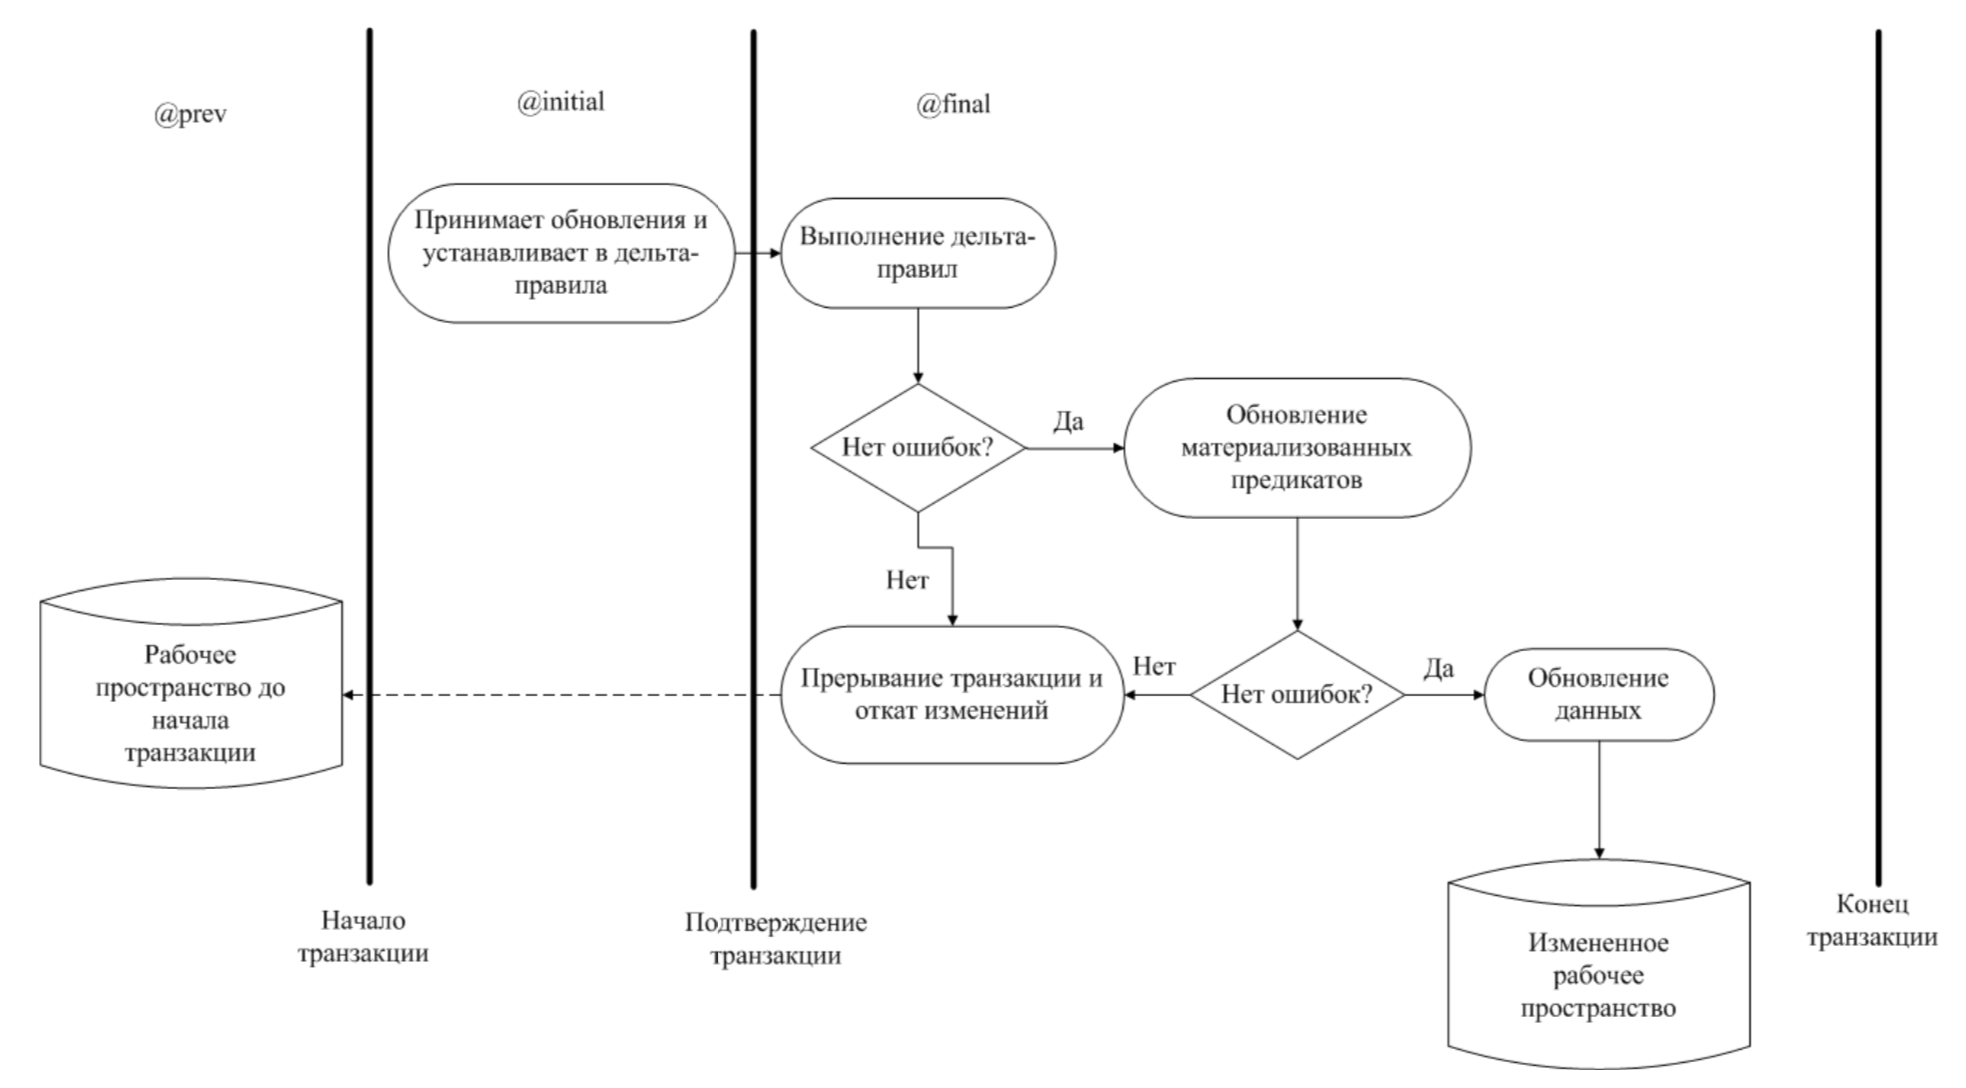
\includegraphics[scale=0.35]{transaction.png}
  	\caption{Жизненный цикл транзакции}
  	\label{fig:technology:logiql:transaction}
  \end{figure}
\end{landscape}

\subsubsection{Бизнес-правила и агрегация}
\label{sec:technology:logiql:aggregations}

Теперь рассмотрим пример бизнес-правил в \logiql:

\begin{lstlisting}[language=Prolog]
netsales_u(product, store, day, net) <-
  sales_u(product, store, day, sls),
  returns_u(product, store, day, returns),
  net = sls - returns.

_(product, tunits) <-
  agg<< tunits=total(untis) >>
    sales_u(product, _, _, units).
\end{lstlisting}

Или, примерный аналог \sql:

\begin{lstlisting}[language=SQL]
CREATE VIEW netsales_u AS
SELECT DISTINCT S.product, S.store, S.day,
  S.unit – R.unit AS net
FROM sales_u S, returns_u R
WHERE S.product = R.product and
  S.store = R.store and
  S.day = R.day;
SELECT product, sum(units)
FROM unit_sales
GROUP BY product.
\end{lstlisting}

Здесь видно объявление еще одного предиката под названием \lstinline{netsales_u}, у которого 4 колонки и значение последней колонки вычисляется как разница значений из других предикатов. Опять же, если говорить в терминах языка \logiql, то определение будет звучать так: для всех записей с фиксированными \lstinline{product}, \lstinline{store}, \lstinline{day} в предикате \lstinline{sales_u} и записей для таких же \lstinline{product}, \lstinline{store}, \lstinline{day} в предикате \lstinline{returns_u} будет существовать запись в предикате \lstinline{netsales_u} с такими же \lstinline{product}, \lstinline{store}, \lstinline{day} и значением последней колонки, равной разнице между \lstinline{sls} и \lstinline{returns}. Другими словами, условие должно выполняться всегда, даже после обновления предикатов \lstinline{sales_u} и \lstinline{returns_u}, что гарантирует нам существование такой записи в \lstinline{netsales_u} \cite{query_language_for_smart_db}.

\subsubsection{Ограничения}
\label{sec:technology:logiql:constraints}

Попробуем наложить ограничения на значения в \logiql:

\begin{lstlisting}[language=Prolog]
sales_u[product, store, day] = unit ->
  string(product),
  string(store),
  datetime(day),
  int(unit).

sales_u[product, store, day] = unit ->
  product_catalog(product).

returns_u[product, store, day] = ret,
sales_u[product, store, day] = sls ->
  ret <= sls.
\end{lstlisting}

Или, аналог в \sql:

\begin{lstlisting}[language=SQL]
CREATE TABLE sales_u
(
  product VARCHAR(15) NOT NULL,
  store VARCHAR(20) NOT NULL,
  day DATETIME NOT NULL,
  unit INT NOT NULL,
  PRIMARY KEY (product, store, day),
  FOREIGN KEY (product)
    REFERENCES product_catalog(product)
);
\end{lstlisting}

В этом листинге появляется синтаксис с \lstinline{[...]}. Это определяет предикат типа ключ-значение. То, что находится в \lstinline{[]} является ключом, после знака равенства определяется значение. Вообще говоря, значение может быть не одно. В этом случае синтаксис немного изменится: \lstinline{some_predicate(key1, key2; val1, val2)}.

Фактически, \lstinline{sales_u} по-прежнему является предикатом с 4 колонками, но он функционально зависим. И если попытаться добавить еще одну запись с теми же \lstinline{product}, \lstinline{store}, \lstinline{day}, но с другим значением \lstinline{unit}, выбросится ошибка \lstinline{Constraint Violation}. Более того, такая нотация позволяет воспринимать этот предикат как функциональный, что при большом количестве предикатов в большом приложении упрощает задачу композиции различных предикатов. Итак, в примере указывается, что если в \lstinline{sales_u} имеется запись для некоторого \lstinline{product}, то такой \lstinline{product} должен находится в предикате \lstinline{product_catalog}. Аналогично, если для некоторых \lstinline{product}, \lstinline{store}, \lstinline{day} существуте запись в соответствующих предикатах,то обязательно должно выполняться \lstinline{ret <= sls}. Иначе, опять же, будет ошибка \lstinline{Constraint Violation}. Такие ограничения будут проверены каждый раз при обновлении записей в предикатах, причем лишь в тех, в которых это имеет смысл.
Среди преимуществ ограничений можно выделить следующие:
\begin{enumerate}
  \item Поддерживается подход «дизайн по контракту», согласно которому мы предполагаем, что ограничения выполняются всегда и нам не нужно их проверять самим. На выходе получаются более читабельные программы.
  \item Не позволяют пользователям выполнять операции, которые нарушают бизнес-правила.
  \item Автоматически расширяют предикаты для удовлетворения системы ограничений. Это ключ к интеграции с оптимизаторами.
\end{enumerate}

Рассмотрим еще один небольшой пример использования ограничений и покажем, насколько мощными они могут быть. Пусть существуют следующие предикаты:

\begin{lstlisting}[language=Prolog]
node(n), node_id(n:uuid) -> string(uuid).
color(c), color(c:color_name) -> string(color_name). edge(u, v) -> node(u), node(v).
color_of[n] = c -> node(n), color(c).
node(n) -> color_of[n] = _.
edge(x, y), color_of[x] = c, color_of[y] = c -> x = y.
\end{lstlisting}

Здесь указаны необходимые предикаты для вершины, ребра и цвета вершины графа. Кроме того, наложено ограничения о том, что каждая вершина должна иметь некоторый цвет и никакие две смежные вершины не могут иметь одинаковый цвет. А теперь с помощью \LB это легко подключается к оптимизатору (например, \emph{Gurobi}), который может найти минимальную возможную раскраску графа. Это достигается лишь одной строкой:

\begin{lstlisting}[language=Prolog]
lang:solver:variable(`color_of).
\end{lstlisting}

Этот пример показывает простую связь между декларативным программированием и программированием в ограничениях \cite{logiql_vs_datalog}.

\subsubsection{Триггеры, события}
\label{sec:technology:logiql:triggers_events}

Рассмотрим триггеры и события на языке \logiql.

\begin{lstlisting}[language=Prolog]
^sales_u[product, store, day] = new_units <-
  +sales_line[_, product, store, day] = line_untis,
  sales_u@prev[product, store, day] = units,
  new_units = line_units + units.
\end{lstlisting}

Или, аналог в \sql:

\begin{lstlisting}[language=SQL]
CREATE TRIGGER update_sales ON sales_line
AFTER INSERT BEGIN
UPDATE sales_u
SET sales_u.units = inserted.units + sales_u.units
FROM sales_u, inserted
WHERE sales_u.product = inserted.product and
  sales_u.store = inserted.store and
  sales_u.day = inserted.day
END;
\end{lstlisting}

Приведенный листинг явно показывает краткость записи в \logiql. Данное правило при каждом добавлении записи в \lstinline{sales_line} при выполнении указанного условия будет обновлять значение в предикате \lstinline{sales_u}. Здесь используется так называемое «дельта правило» (со знаком «\lstinline{+}» и «\lstinline{^}»), которое в данном случае говорит о вставке записи. Так же существует дельта правила на обновление (\lstinline{upsert}) и удаление. \lstinline{@prev} здесь указывает на одну стадию жизненного цикла транзакции (в конкретном случае – до начала транзакции).
Единственные отрицательные стороны данного (по сравнению с \sql) подхода в том, что события не могут вызывать другие события и события также не могут изменять схему \cite{query_language_for_smart_db}.

\subsubsection{Queries и Spreads}
\label{sec:technology:logiql:queries_spreads}

В \logiql все запросы разделяются на \emph{queries} и \emph{spreads}. Первые используются для получения информации (значений предикатов, агрегированной информации), вторые – для обновления информации. Пример из главы про бизнес-правила является типичным примером \emph{query}, где может происходить выборка по количеству проданных продуктов, а пример из предыдущей главы служит как \emph{spread} – с помощью него можно обновлять значения в предикатах при изменении в других.
Видно наглядно, что на языке \logiql описание предикатов и правил смотрятся логичнее, проще и понятнее, чем в \sql. Эта лаконичность также является одной из особенностей этого языка.
Выделим ключевые моменты языка \logiql:

\begin{enumerate}
  \item декларативный язык;
  \begin{itemize}
    \item нормализация ключ-значение (6 нормальная форма);
    \item булева логика - не содержит нулевых записей;
    \item семантика множеств;
  \end{itemize}
  \item выразительный;
  \begin{itemize}
    \item правила/запросы аналогичны \sql views и запросам;
    \item событийные правила с той же смысловой нагрузкой, что и в \sql, но проще в реализации;
    \item делает возможным оптимизации, машинное обучение легковстраиваевым \cite{query_language_for_smart_db}.
  \end{itemize}
\end{enumerate}

\subsubsection{Move computation to data, not vice versa}
\label{sec:technology:data_to_computation}

\LB придерживается следующего принципа: "Move com\-pu\-ta\-tion to data, not vice versa". Это достигается с помощью двух составляющих:

\begin{enumerate}
  \item dataflow graph (граф потока данных);
  \item incremental view maintenance (поэтапное поддержание представлений).
\end{enumerate}

Идея \emph{dataflow graph} (рисунок \ref{fig:technology:data_to_computation:dataflow_graph}) была использована в 1980-90 гг. в оптимизации компиляторов. Представление программы в виде такого графа вместо ее императивной структуры (сверху-вниз и слева-направо) позволяет автоматически ее параллелить. Например, для простой программы следующего вида можно составить граф, представленный на рисунке \ref{fig:technology:data_to_computation:dataflow_graph_parallel}, на котором также можно выделены операции, которые можно запустить параллельно (разные ветви графа):

\begin{lstlisting}[language=Pascal]
x := a * b;
y := 5 + x;
z := c + a;
\end{lstlisting}

\begin{figure}
	\centering
	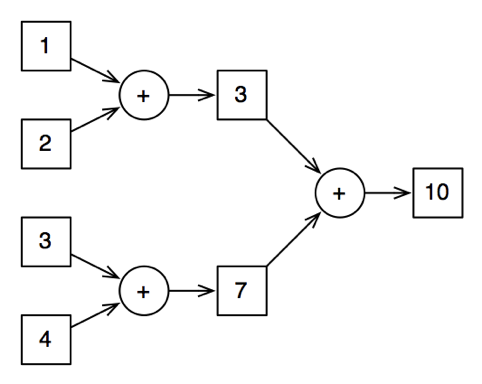
\includegraphics[scale=0.9]{dataflow_graph.png}
	\caption{Пример графа потока данных}
	\label{fig:technology:data_to_computation:dataflow_graph}
\end{figure}

\begin{figure}
	\centering
	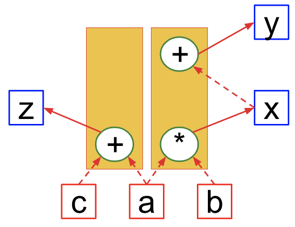
\includegraphics[scale=1.0]{dataflow_graph_parallel.png}
	\caption{Пример возможности параллелизации программы с помощью графа потока данных}
	\label{fig:technology:data_to_computation:dataflow_graph_parallel}
\end{figure}

Если же в примере заменить операцию присвоения на символ стрелки (\lstinline{<-}), то получится костяк программы на \logiql:

\begin{lstlisting}[language=Prolog]
x <- a * b.
y <- 5 + x.
z <- c + a.
\end{lstlisting}

Язык создан таким образом, чтобы среда выполнения могла построить такой dataflow graph. Затем по такому графу выполняется \emph{incre\-men\-tal view maintenance}. Он нужен для того, чтобы уменьшить количество пересчитываемых данных, в этом также помогает уже построенный dataflow graph. К примеру, из приведенного фрагмента программы (на рисунке \ref{fig:technology:data_to_computation:dataflow_graph}) можно понять, что при обновлении переменной \lstinline{c} необходимо лишь пересчитать значение переменной \lstinline{z}, а если поменялось значение \lstinline{a}, тогда нужно провести вычисления для всех переменных (\lstinline{x}, \lstinline{y}, \lstinline{z}).

Кроме того, в некоторых случаях даже обновление переменных не требует пересчета всей ее формулы. Например, в случае суммы \lstinline{a := x + y + z} изменение одного аргумента (\lstinline{y}) влечет лишь обычное изменение целевой переменной \lstinline{a} без дополнительного знания значений остальных аргументов (\lstinline{x} и \lstinline{z}).

Что же со всем этим делает платформа? На самом деле, \emph{вершины-данные} представляются как предикаты (аналог таблиц в \sql), а \emph{вершины-функции} - это запросы или вызовы оптимизационных решателей. Дальнейшее использование такого представления не вызывает лишних вопросов.

